\documentclass[a4paper,11pt]{article}

\usepackage{tikz}
\usetikzlibrary{calc}

\usepackage{graphicx}

\newcommand{\class}[1]{{\texttt #1}}
\newcommand{\method}[1]{{\texttt #1}}
\newcommand{\package}[1]{{\textsf #1}}

\begin{document}

\title{Updated overview and present status of work on the multi-type
  tree sampler}

\author{Tim Vaughan, Denise K\"uhnert, Alexei Drummond}

\maketitle

\section{Introduction}

We discuss here the current status and future goals of the project
to implement a multi-type (or coloured) tree distribution sampler
within the BEAST framework. Such a sampler will enable us to infer
parameters under the assumption of sophisticated population genetics
and epidemiological models.

Currently, the sampler is implemented as an add-on called
\package{ColouredTree}. The eventual goal, however, is to integrate the
sampler into the production BEAST 2 code.


\section{Overview of framework}

To date, we have a working framework for the sampler in place.  The
best place to go for the nitty-gritty details of the sampler is the
JavaDoc output from the ColouredTree source.  What follows is
therefore only a cursory outline of the framework.


\subsection{The ColouredTree plugin}

The main class of the sampler is \class{ColouredTree}, which derives
from \class{Plugin}. This class is essentially just a wrapper around a
\class{Tree} input and four \class{Parameter} inputs which together
contain the information about the tree topology and the distribution
of migration/infection events along its branches.
Figure~\ref{fig:treeComposition} contains a schematic illustrating
this structure.

\begin{figure}
\centering
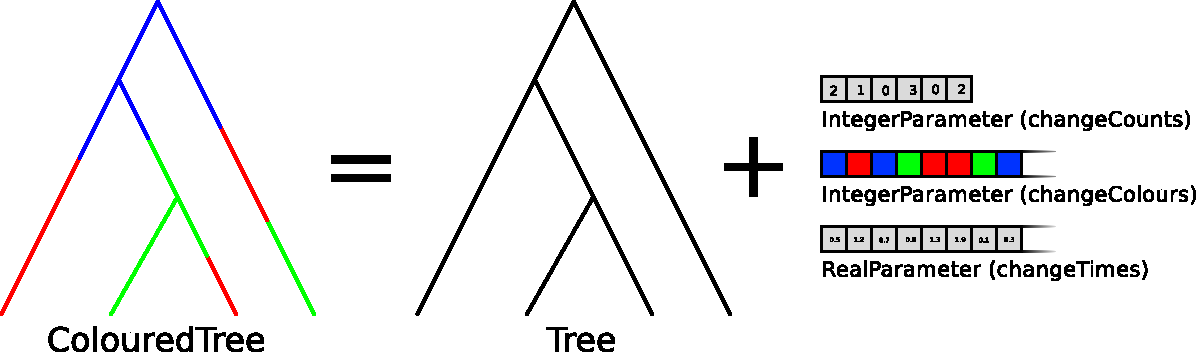
\includegraphics[width=\textwidth]{treeComposition.pdf}
\caption{Schematic representation of how the multi-type tree plugin
  \class{ColouredTree} represents the type/deme/colour information
  along each branch.  Note that the types at each of the nodes are
  also recorded, although these are completely specified by the list
  of change times and colours.}
\label{fig:treeComposition}
\end{figure}

Besides this primary function, \class{ColouredTree} contains public
methods necessary for obtaining information about the multi-type tree
it represents.  At the most basic level this includes methods which
return the number of migration events along each branch, as well as
the type and time of each of these events.

Noteably, \class{ColouredTree} does \emph{not} contain the methods
necessary for modifying any of the details of these events.  This is
due to the restriction imposed by BEAST that only methods belonging to
classes derived from \class{Operator} are permitted to alter instances
of \class{StateNode} such as \class{Parameter}.  For this reason,
many of these methods (which were originally contained in
\class{ColouredTree}) have been moved to \class{ColouredTreeOperator}.

There is one exception to this rule: the \method{initFromFlatTree()}
method, which avoids this difficulty by calling the more primitive
methods belonging to \class{ColouredTreeModifier} which is a special
subclass of \class{ColouredTreeOperator} constructed specifically for
this purpose.

\subsection{The ColouredTreeOperator plugin}

The abstract \class{ColouredTreeOperator} class is designed to be
subclassed by operators intended to modify \class{ColouredTree}
configurations.  It includes all of the methods one might otherwise
expect to see in \class{ColouredTree}, including primitive setters
like \method{setChangeColour()}, \method{setChangeTime()} and
\method{setChangeCount()}, togther with composite and more useful
methods such as \method{addChange()}.

Importantly, \class{ColouredTreeOperator} now also defines a method
\method{setRoot()} which should be used in place of the method of the
same name defined by the \class{Tree} class to change the root node of
a multi-type tree topology.  The reason behind this is that
\class{Tree.setRoot()} has recently begun to alter the ID numbers of
nodes in the tree to ensure that the root node is always given the ID
$n-1$.  The method \class{ColouredTreeOperator.setRoot()} updates the
data in \class{ColouredTree} to reflect this change.

As mentioned above, there is a special subclass of the abstract
\class{ColouredTreeOperator} named \class{ColouredTreeModifier} which
is intended to be directly instantiated and used in methods which need
to be able to modify \class{ColouredTree} objects but for which direct
inclusion in \class{ColouredTreeOperator} does not make sense from a
structural point of view.  This includes the
\class{ColouredTree.initFromFlatTree()} method mentioned previously,
as well as methods implementing \class{StateNodeInitialiser} such as
\class{StructuredCoalescentColouredTree}. (Ordinarily, a
\class{StateNodeInitialiser} sets the initial values of a
\class{StateNode} using its constructor.  This is not an ideal
approach to constructing complex multi-type tree objects, however,
which are much easier to construct in an incremental fashion.

\subsection{The ColouredTreeDistribution plugin}

The \class{ColouredTreeDistribution} plugin is another abstract class,
in this case designed to be subclassed by likelihoods and priors over
the multi-type tree space.  Only two such distributions presently
exist: a structured coalescent distribution named
\class{StructuredCoalescentLikelihood} and Denise's birth-death model
likelihood.

\subsection{The MigrationModel plugin}

This plugin is intended to be the equivalent of
\class{SubstitutionModel} for multi-type trees. Its primary contents
are a migration rate matrix and a vector of deme population sizes. It
also contains a set of helper methods which calculate eigenvalue
decompositions of the rate matrix and use this to calculate transition
probabilities between demes along lineages. It is derived from
\class{CalculationNode} as the eigenvalue decomposition must be
recalculated whenever the migration rates and/or population sizes are
altered.


\subsection{The ColouredTreeFromNewick plugin}

This plugin is useful for initialising \class{ColouredTree} objects
using a tree specification given in Newick format.  Colour changes are
specified using single-child nodes and the colours themselves are
specified as traits on the node below the branches they refer to.
Internally, this plugin uses the \class{TreeParser} plugin in
combination with \class{ColouredTree.initFromFlatTree()}.  (Previously
this used a complex arrangement of methods which Denise was forced to
come up with due to short-commings in my original code.)

\section{Operators for multi-type trees}

The operators which are responsible for sampling from the multi-type
tree proposal distribution are very similar to those already defined
for sampling from traditional rooted tree distributions.  There are
differences, however, and these are enough to require at least trivial
reimplementation each of the original BEAST tree operators.

\subsection{Special considerations}

The differences hinted at above are primarily to do with the fact that
multi-type trees have an additional level of state information
associated with each branch, and that any modification of the tree
must take this additional state information into consideration or else
an inconsistent or otherwise invalid multi-type tree may result.

Consider a branch corresponding to a lineage in a particular deme, for
example. If an operator alters the tree topology by reconnecting this
branch to some other point on the tree, it may connect the tree
directly to a lineage in another deme if the geographical locations
associated with the branches involved are not explicitly taken into
account.  Similarly, if the height of a node on the tree is adjusted
without considering the timing of migration events, the repositioned
node may find itself above or below a migration event on one of its
connected branches---another obviously invalid situation.

There are a number of possible approaches to dealing with problems
like these.  Firstly, we can \emph{constrain} the modifications
introduced by the existing \class{Tree} operators to ensure the
proposed trees are valid multi-type trees.  Another alternative is to
allow the operators to do what they will, but to then \emph{discard}
any proposal which does not meet the validity criteria. Both of these
approaches have the advantage that they require only trivial
modification of the existing suite of operators.  There are at least
two drawbacks, however: 1) we expect the mixing rates to be quite
slow---especially as the number of types/demes and the frequency of
type-shift/migration events increase, and 2) these modified operators
do not explore the possible migration paths meaning that special
additional operators must be constructed specifically for this purpose.

The third alternative, and the approach that we have chosen in most
cases to pursue, is to have the operators modify both the components
of \class{Tree} and \class{ColouredTree} simultaneously: allowing both
traditional tree modifications and modifications to the migratory
paths in a single move.

\subsection{Implemented operators}

Below is a brief description of each of the operators which have been
implemented so-far.

\subsubsection{ColouredWilsonBaldingRandom}

This is the first of two operators based the branch-swapping move
operator first proposed by Wilson and Balding \cite{Wilson1998} and
later modified by Drummond et al. \cite{Drummond2002}. The tree
topology changes invoked by the non-typed move are shown in figure
\ref{fig:WBmove}.  These changes simply involve selecting a subtree at
random, dissolving the branch connecting the subtree to the rest of
the tree then creating a replacement branch to some other location on
the tree.


\begin{figure}
\hspace{-1cm}
\begin{tikzpicture}
\coordinate (leaf1) at (-3,0);
\coordinate (leaf2) at (-1,0);
\coordinate (leaf3) at (1,0);
\coordinate (leaf4) at (3,0);
\coordinate (internal) at (0,1);
\coordinate (root) at (0,5);

\draw (leaf2)--(internal) node[below]{$i$}--(leaf3);
\draw (leaf1) node[right=3pt]{}--(root) node[left=3pt]{} node[right=3pt]{$j_p$}--(leaf4) node[right]{$j$};
\fill (root) circle (0.05);
\fill (internal) circle (0.05);
\fill (leaf1) circle (0.05);
\fill (leaf2) circle (0.05);
\fill (leaf3) circle (0.05);
\fill (leaf4) circle (0.05);

% AUCTeX preview can't handle this:
\coordinate (source) at ($(leaf1)!0.6!(root)$);
\coordinate (dest) at ($(leaf4)!0.5!(root)$);
\draw (internal)--(source) node[left]{$i_p$};
\draw [dashed] (internal)--(dest) node[right]{$i_{p'}$};
\fill (source) circle (0.05);
\fill (dest) circle (0.05);

\draw (-3,5) node{(a)};

\end{tikzpicture}\hspace{1cm}\begin{tikzpicture}
\coordinate (leaf1) at (-2,0);
\coordinate (leaf2) at (0,0);
\coordinate (leaf3) at (4,0);
\coordinate (oldRoot) at (2,3);
\coordinate (newRoot) at (0,5);

\draw (leaf2) node[left]{$i_s$}--(oldRoot) node[right]{$j$}--(leaf3);
\draw [dashed] (leaf1) node[left]{$i$}--(newRoot)--(oldRoot);

% AUCTeX preview can't handle this:
\coordinate (source) at ($(leaf2)!0.6!(oldRoot)$);
\draw [color=gray](leaf1)--(source);
\fill (source) circle (0.05);
\draw (source) node[right=3pt]{$i_p$};
\draw (newRoot) node[right=3pt]{$i_{p'}$};

\fill (oldRoot) circle (0.05);
\fill (newRoot) circle (0.05);
\fill (leaf1) circle (0.05);
\fill (leaf2) circle (0.05);
\fill (leaf3) circle (0.05);

\draw (-2,5) node{(b)};

\end{tikzpicture}
\caption{The two kinds of tree topology changes invoked by the
  modified Wilson-Balding moves: (a) moves which do not alter the root
  and (b) those which do.  In both of these figures, the dashed line
  represents a new branch to be created and coloured/typed.}
\label{fig:WBmove}
\end{figure}

 In order to cope with multi-typed trees, the
\class{ColouredWilsonBaldingRandom} operator simply dissolves the type
information along with the deleted branch, then generates a completely
new migration path along the newly created connecting branch.  In the
case of this particular operator, the proposal distribution for the
new path is simply a fixed rate continuous time random walk between
the available demes, starting at the deme corresponding to the top of
the chosen subtree.  In the case that the deme at the end of the walk
does \emph{not} match the deme at the new connection point ($i_{p'}$
in the figure), the entire move is discarded.  Note that the rate of
the process used to generate the new path is not inferred (it has no
physical meaning) but is instead simply a tuning parameter of the operator.

\subsubsection{ColouredWilsonBalding}

The \class{ColouredWilsonBalding} operator is a more sophisticated
variant of the last operator.  It differs only in that where that
operator used a fixed rate random walk to generate the migratory path
along the new branch, \class{ColouredWilsonBalding} uses the combined
uniformization/forward-backward algorithm of Fearnhead and Sherlock
\cite{Fearnhead2006} to sample migration paths from a provided
\class{MigrationModel} conditional on the location/deme/type at
\emph{both} ends of the new branch.  This operator therefore has in
general a significantly higher per move acceptance probability than
its simpler cousin, although this comes at the expense of a more
computationally complex proposal algorithm.

\subsubsection{ColouredTreeScale}

This operator is a trivial extension of the \class{TreeScale} operator
and simply multiplies the height of all coalescence nodes and lineage
migrations in the tree by a constant scale factor.

\subsubsection{ColouredSubtreeSlide}

This operator extends \class{SubtreeSlide} in the same way that the
Wilson-Balding operator is extended by
\class{ColouredWilsonBaldingRandom}.  The original subtree slide
involves selecting a branch connecting a subtree to the rest of the
tree, dissolving that branch, then reconnecting the subtree to a point chosen
uniformly along the branch to which the subtree was originally joined.  In the
multi-type extension to this operator, the migratory path along the
newly created branch is generated using a constant rate random walk as
described above.

\subsubsection{ColouredUniform}

This operator is an extension to the existing \class{Uniform} tree
operator which ensures the validity of its application to multi-type
trees by constraining the range of the uniform adjustment of node
heights. 

\section{Work still to complete}

Although the sampler is already functional, there are a number of loose ends
still remaining.

\subsection{Operators to implement}

While we already have a suite of operators which together are in
principle capable of exploring the complete space of multi-type trees,
we expect the following additions to markedly improve the overall
mixing rate of the sampler:
\begin{enumerate}
\item extension of the \class{ColouredTreeScaler} to provide a general
  up-down scaling operator for the simultaneous scaling of the
  multi-type tree height and other model parameters, and
\item implementation of multi-type tree versions of the narrow and
  wide exchange operators to allow for bolder tree topology changes,
  which are particularly useful during the burn-in phase.
\end{enumerate}

\subsection{Performance testing}

In order to assess the performance (i.e. rate of mixing per unit CPU
time) of the completed sampler, we intend to directly compare it to
the sampler detailed by Ewing et al.~\cite{Ewing2004}.  That sampler
uses the \emph{discarding} approach to apply the regular BEAST tree
moves to multi-type trees, with the addition of two operators which
exclusively modify the type information.  We intend to implement these
additional moves in BEAST, enabling us to perform the comparison on
using whichever set of data we choose.

\subsection{Additional goals}

Once we are happy with the overall performance and stability of the
sampler, we intend to publish a methods paper (perhaps in BMC
Bioinformatics) detailing the new operators and announcing the demise
of Migrate.

%\bibliography{virus_papers}
%\bibliographystyle{unsrt}

\begin{thebibliography}{1}

\bibitem{Wilson1998}
I.~J. Wilson and D.~J. Balding.
\newblock Genealogical inference from microsatellite data.
\newblock {\em Genetics}, 150(1):499--510, Sep 1998.

\bibitem{Drummond2002}
Alexei~J. Drummond, Geoff~K. Nicholls, Allen~G. Rodrigoa, and Wiremu Solomonc.
\newblock Estimating mutation parameters, population history and genealogy
  simultaneously from temporally spaced sequence data.
\newblock {\em Genetics}, 161:1307, 2002.

\bibitem{Fearnhead2006}
Paul Fearnhead and Chris Sherlock.
\newblock An exact Gibbs sampler for the Markov-modulated Poisson process.
\newblock {\em Journal of the Royal Statistical Society: Series B}, 68:767,
  2006.

\bibitem{Ewing2004}
Greg Ewing, Geoff Nicholls, and Allen Rodrigo.
\newblock Using temporally spaced sequences to simultaneously estimate
  migration rates, mutation rate and population sizes in measurably evolving
  populations.
\newblock {\em Genetics}, 168(4):2407--2420, Dec 2004.

\end{thebibliography}

\end{document}
